% TaskCalendar — System Report
% Compile with: pdflatex taskcalendar-report.tex (run twice for TOC)
% Optional: latexmk -pdf taskcalendar-report.tex
%
% Required packages (all standard in TeX Live / MiKTeX):
%   geometry hyperref graphicx tikz xcolor enumitem booktabs listings
%   fancyhdr titlesec amsmath amssymb amsfonts caption float

\documentclass[11pt,a4paper]{article}

\usepackage[utf8]{inputenc}
\usepackage[T1]{fontenc}
\usepackage{lmodern}
\usepackage[margin=2.4cm]{geometry}
\usepackage{graphicx}
\usepackage{xcolor}
\usepackage{tikz}
\usetikzlibrary{shapes.geometric, arrows.meta, positioning, fit, calc, backgrounds, shadows.blur}
\usepackage{enumitem}
\usepackage{booktabs}
\usepackage{listings}
\usepackage{caption}
\usepackage{float}
\usepackage{titlesec}
\usepackage{fancyhdr}
\usepackage{amsmath}
\usepackage{hyperref}

% ── Colours (match the TaskCalendar brand) ────────────────────────────────
\definecolor{tcAccent}{HTML}{F97316}      % orange-500
\definecolor{tcAccentSoft}{HTML}{FED7AA}  % orange-200
\definecolor{tcInk}{HTML}{0F172A}         % slate-900
\definecolor{tcMuted}{HTML}{64748B}       % slate-500
\definecolor{tcLight}{HTML}{E2E8F0}       % slate-200
\definecolor{tcBg}{HTML}{F8FAFC}          % slate-50
\definecolor{tcEmerald}{HTML}{22C55E}
\definecolor{tcSky}{HTML}{0EA5E9}
\definecolor{tcViolet}{HTML}{8B5CF6}
\definecolor{tcRose}{HTML}{F43F5E}

\hypersetup{
  colorlinks=true,
  linkcolor=tcAccent,
  urlcolor=tcAccent,
  citecolor=tcAccent,
  pdftitle={TaskCalendar — System Report},
  pdfauthor={Securovix Ltd},
}

% ── Section styling ───────────────────────────────────────────────────────
\titleformat{\section}
  {\Large\bfseries\color{tcInk}}
  {\thesection}{0.7em}{}
\titleformat{\subsection}
  {\large\bfseries\color{tcInk}}
  {\thesubsection}{0.6em}{}
\titleformat{\subsubsection}
  {\normalsize\bfseries\color{tcAccent}}
  {\thesubsubsection}{0.5em}{}

% ── Headers / footers ─────────────────────────────────────────────────────
\pagestyle{fancy}
\fancyhf{}
\fancyhead[L]{\small\color{tcMuted}TaskCalendar — System Report}
\fancyhead[R]{\small\color{tcMuted}Securovix Ltd}
\fancyfoot[C]{\small\thepage}
\renewcommand{\headrulewidth}{0.4pt}
\renewcommand{\headrule}{\hbox to\headwidth{\color{tcLight}\leaders\hrule height \headrulewidth\hfill}}

% ── Code listings (TypeScript, SQL) ───────────────────────────────────────
\lstdefinelanguage{TypeScript}{
  keywords={const,let,var,function,return,if,else,async,await,export,import,from,interface,type,as,typeof,boolean,string,number,null,undefined,Promise,extends,implements,class,new,this,for,while,switch,case,break,default,Record},
  keywordstyle=\color{tcAccent}\bfseries,
  ndkeywords={true,false,console},
  ndkeywordstyle=\color{tcSky}\bfseries,
  identifierstyle=\color{tcInk},
  sensitive=true,
  comment=[l]{//},
  morecomment=[s]{/*}{*/},
  commentstyle=\color{tcMuted}\itshape,
  stringstyle=\color{tcEmerald},
  morestring=[b]',
  morestring=[b]",
  morestring=[b]`,
}
\lstdefinestyle{tcSnippet}{
  basicstyle=\ttfamily\footnotesize,
  backgroundcolor=\color{tcBg},
  frame=single,
  framerule=0pt,
  rulecolor=\color{tcLight},
  xleftmargin=0.7em,
  framexleftmargin=0.7em,
  framexrightmargin=0.7em,
  framextopmargin=0.4em,
  framexbottommargin=0.4em,
  breaklines=true,
  showstringspaces=false,
  columns=fullflexible,
  keepspaces=true,
  language=TypeScript,
}
\lstset{style=tcSnippet}

% ── TikZ styles ───────────────────────────────────────────────────────────
\tikzset{
  tcBox/.style={
    rectangle, rounded corners=4pt, draw=tcLight, line width=0.6pt,
    fill=white, minimum height=1.0cm, minimum width=2.3cm,
    align=center, font=\small, drop shadow={opacity=0.08},
  },
  tcAccentBox/.style={
    tcBox, draw=tcAccent, fill=tcAccentSoft!40, text=tcInk,
  },
  tcMutedBox/.style={
    tcBox, fill=tcBg, draw=tcLight,
  },
  tcArrow/.style={
    -{Stealth[length=4pt]}, line width=0.9pt, draw=tcMuted,
  },
  tcAccentArrow/.style={
    tcArrow, draw=tcAccent,
  },
  tcGroup/.style={
    draw=tcLight, dashed, rounded corners=4pt, inner sep=10pt,
  },
}

% ── Title block ───────────────────────────────────────────────────────────
\title{
  \vspace{-1.5cm}
  {\color{tcAccent}\Huge\bfseries TaskCalendar}\\[0.4em]
  {\Large\color{tcInk} System Report}\\[0.3em]
  {\large\color{tcMuted}Architecture, CRM, Automation, and Chat-bot Integrations}
}
\author{Securovix Ltd \\[2pt] \small\href{mailto:info@securovix.com}{info@securovix.com}}
\date{20 May 2026}

% ──────────────────────────────────────────────────────────────────────────
\begin{document}
\maketitle
\thispagestyle{empty}

\begin{abstract}
\noindent
TaskCalendar is a multi-tenant SaaS that consolidates project management,
a sales CRM, automation, AI assistance, and chat-bot control into a
single workspace. This report documents the system end-to-end with
emphasis on the \textbf{Clients} module and the \textbf{Automation engine}
— the two surfaces that differentiate the product from pure
task-management tools. We cover the data model, the runtime
architecture, the role of every Supabase Edge Function, the chat-bot
adapters on Telegram and WhatsApp, the dashboards built on top, the
subscription plan gating, and the security posture. Diagrams accompany
every section.
\end{abstract}

\vfill
\begin{center}
\small\color{tcMuted}
\textit{Last updated 20 May 2026. Built on Vite + React 18, Supabase
(PostgreSQL + Auth + Edge Functions), Firebase Auth bridge,
OpenAI gpt-4o-mini, Stripe Billing, Meta WhatsApp Cloud API,
Telegram Bot API, Cloudflare Turnstile, framer-motion, Recharts.}
\end{center}

\newpage
\tableofcontents
\newpage

% ──────────────────────────────────────────────────────────────────────────
\section{Introduction}

TaskCalendar's stated goal in the landing copy is to be \emph{``one
workspace for teams that ship.''} Concretely it delivers:

\begin{enumerate}[leftmargin=*,itemsep=2pt]
  \item Project / task management — Kanban boards, calendar, timeline,
    workspaces, custom columns, file attachments, task locks, comments,
    mentions, and a notification inbox.
  \item A sales CRM — clients, multi-pipeline deals, lead forms with
    bot-protection, lead scoring, client categories, contacts, notes,
    file uploads, deal-scoped activity logging, and analytics
    dashboards.
  \item Automation — declarative \emph{when X happens, do Y} recipes
    with eight triggers and nine action handlers, plus AI Blocks, an
    AI Sales Agent, and Slack-driven triggers.
  \item Chat-bot integrations — Telegram and Meta WhatsApp bots that
    let an authenticated user create workspaces, projects, tasks,
    clients, and CRM activities via natural-language messages.
  \item Integrations — Google Calendar / Meet / Gmail (per-user OAuth),
    Slack (org-level OAuth + Events API), Stripe Billing, EmailJS
    fallback notifications.
  \item Subscription gating — four tiers (Starter, Basic, Advanced,
    Premium) with a 28-day full-feature trial.
\end{enumerate}

This report is written to be \textbf{self-contained}: a reader who has
never seen the codebase should be able to understand what each
component does, how data flows, and where each behaviour is enforced.

% ──────────────────────────────────────────────────────────────────────────
\section{High-level architecture}

\subsection{Runtime view}

The frontend is a Vite-built React 18 single-page app served from
Vercel. The backend is Supabase: PostgreSQL with Row-Level Security,
Realtime channels, Storage, and Deno-based Edge Functions. Identity is
Firebase Auth bridged into Supabase JWTs. Everything writes through
either the user's Supabase JWT (RLS-gated) or a server-side
security-definer RPC.

\begin{figure}[H]
\centering
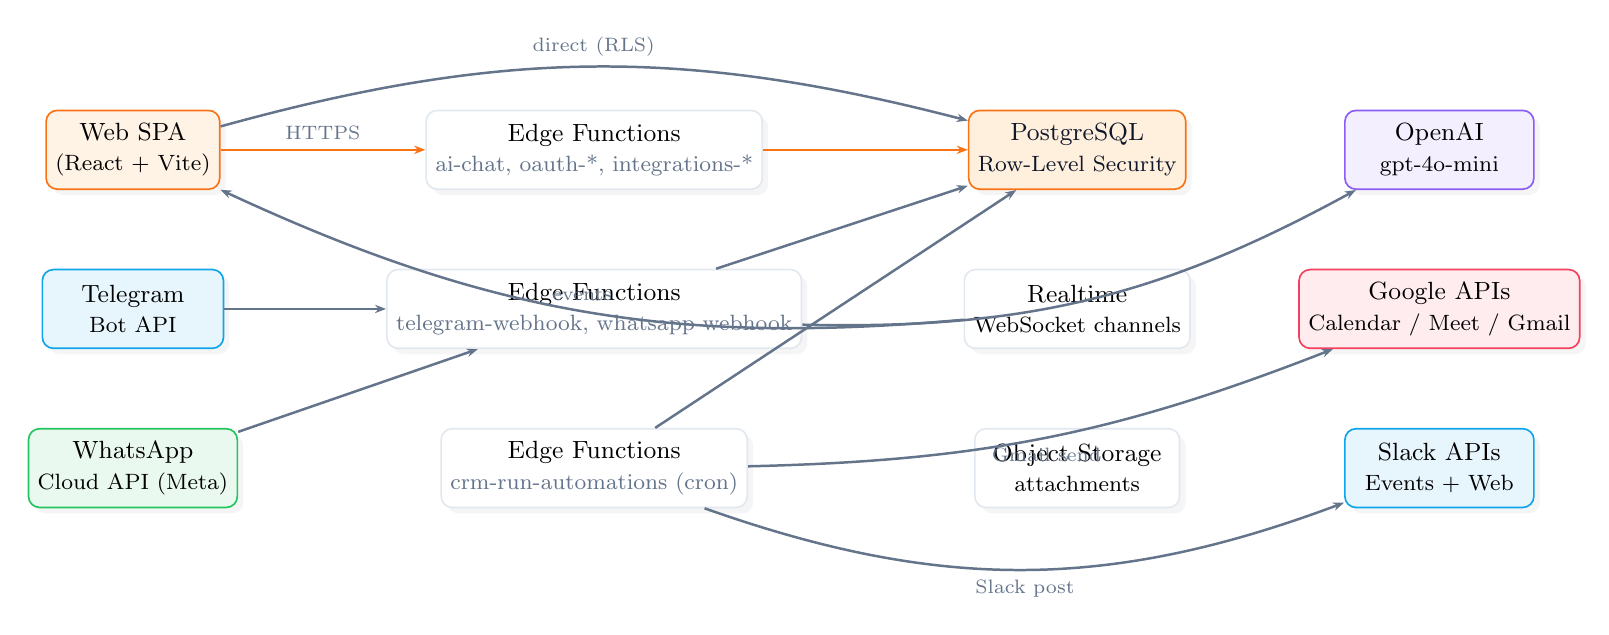
\begin{tikzpicture}[node distance=1.0cm and 1.2cm]

  % Clients (browsers + bots)
  \node[tcBox, fill=tcAccentSoft!30, draw=tcAccent, minimum width=2.2cm] (browser) {Web SPA\\\footnotesize (React + Vite)};
  \node[tcBox, draw=tcSky, fill=tcSky!10, below=of browser] (telegram) {Telegram\\\footnotesize Bot API};
  \node[tcBox, draw=tcEmerald, fill=tcEmerald!10, below=of telegram] (whatsapp) {WhatsApp\\\footnotesize Cloud API (Meta)};

  % Edge functions cluster
  \node[tcBox, right=2.6cm of browser, minimum width=2.4cm] (fnApi) {Edge Functions\\\footnotesize {\color{tcMuted}ai-chat, oauth-*, integrations-*}};
  \node[tcBox, below=of fnApi, minimum width=2.4cm] (fnBot) {Edge Functions\\\footnotesize {\color{tcMuted}telegram-webhook, whatsapp-webhook}};
  \node[tcBox, below=of fnBot, minimum width=2.4cm] (fnAuto) {Edge Functions\\\footnotesize {\color{tcMuted}crm-run-automations (cron)}};

  % Supabase
  \node[tcAccentBox, right=2.6cm of fnApi, minimum width=2.6cm] (pg) {PostgreSQL\\\footnotesize Row-Level Security};
  \node[tcBox, below=of pg, minimum width=2.6cm] (realtime) {Realtime\\\footnotesize WebSocket channels};
  \node[tcBox, below=of realtime, minimum width=2.6cm] (storage) {Object Storage\\\footnotesize attachments};

  % External APIs
  \node[tcBox, right=2.0cm of pg, draw=tcViolet, fill=tcViolet!10, minimum width=2.4cm] (openai) {OpenAI\\\footnotesize gpt-4o-mini};
  \node[tcBox, below=of openai, draw=tcRose, fill=tcRose!10, minimum width=2.4cm] (google) {Google APIs\\\footnotesize Calendar / Meet / Gmail};
  \node[tcBox, below=of google, draw=tcSky, fill=tcSky!10, minimum width=2.4cm] (slack) {Slack APIs\\\footnotesize Events + Web};

  % Arrows: browser → edge → DB
  \draw[tcAccentArrow] (browser) -- node[above,font=\scriptsize\color{tcMuted}]{HTTPS} (fnApi);
  \draw[tcAccentArrow] (fnApi) -- (pg);
  \draw[tcArrow] (browser) edge[bend left=15] node[font=\scriptsize\color{tcMuted},above]{direct (RLS)} (pg);

  % Bots → webhook
  \draw[tcArrow] (telegram) -- (fnBot);
  \draw[tcArrow] (whatsapp) -- (fnBot);

  % Webhook → DB + LLM
  \draw[tcArrow] (fnBot) -- (pg);
  \draw[tcArrow] (fnBot) edge[bend right=15] (openai);

  % Cron worker
  \draw[tcArrow] (fnAuto) -- (pg);
  \draw[tcArrow] (fnAuto) edge[bend right=20] node[font=\scriptsize\color{tcMuted},below]{Slack post} (slack);
  \draw[tcArrow] (fnAuto) edge[bend right=10] node[font=\scriptsize\color{tcMuted},below]{Gmail send} (google);

  % Realtime
  \draw[tcArrow] (realtime) edge[bend left=15] node[font=\scriptsize\color{tcMuted},above]{events} (browser);

\end{tikzpicture}
\caption{Runtime topology. The web SPA talks to PostgreSQL directly
under RLS for reads, and to Edge Functions for any action that
requires a service-role write or a third-party API call. Chat bots
deliver inbound messages to their respective webhooks, which share a
common \texttt{\_shared/agent} core for intent parsing and entity
creation.}
\label{fig:runtime}
\end{figure}

\subsection{Multi-tenancy boundaries}

Every domain table carries an \texttt{organization\_id uuid} column,
and every read/write policy joins through a helper
(\texttt{is\_org\_member(p\_org)} for the user's own JWT,
\texttt{is\_org\_member\_for(p\_user\_id, p\_org\_id)} for service-role
callers like the bot webhooks). The organization is the unit of
isolation; one user can belong to multiple organisations via a
\texttt{members[]} JSONB array on \texttt{organizations}.

% ──────────────────────────────────────────────────────────────────────────
\section{The Clients module}

The Clients module is the CRM half of TaskCalendar. It is gated behind
the \texttt{crm} feature flag (Advanced plan and above; see
Section~\ref{sec:plans}).

\subsection{Entity model}

Five tables form the CRM data spine:

\begin{itemize}[leftmargin=*,itemsep=2pt]
  \item \texttt{clients} — companies or individuals. Carries name,
    legal name, industry, \textbf{category} (free text + suggestions),
    type, status, contact details, address, annual revenue,
    employee count, lead score and band, owner, tags, custom fields
    (JSONB).
  \item \texttt{client\_contacts} — humans associated with a client.
    First/last name, title, email, phone, mobile, primary flag.
  \item \texttt{client\_notes} — activity log of kind
    \{note, call, meeting, email, task\}. Carries optional
    \textbf{deal\_id} so a note can be scoped to a specific deal
    (added in migration 089).
  \item \texttt{client\_attachments} — uploaded files referenced by
    Storage path.
  \item \texttt{client\_tasks} — follow-up tasks
    (kind: todo / call / email / meeting / followup). Links optionally
    to a client and/or a deal.
\end{itemize}

Deals live in their own family of tables:

\begin{itemize}[leftmargin=*,itemsep=2pt]
  \item \texttt{deals} — title, value, currency, stage, probability,
    expected/actual close date, owner, source, pipeline, stage id,
    tags, loss reason.
  \item \texttt{pipelines} and \texttt{pipeline\_stages} — admin-
    configurable per organisation. Stage flags
    (\texttt{is\_won}, \texttt{is\_lost}, \texttt{required\_fields},
    \texttt{default\_probability}) drive UX gates such as the Won
    modal.
  \item \texttt{lead\_scoring\_rules} and
    \texttt{lead\_scoring\_thresholds} — rules that compute the
    client's score 0–100 and assign a band (cold/warm/hot).
  \item \texttt{lead\_forms} — public form definitions with
    Cloudflare Turnstile bot-protection and a per-form deduplication
    policy.
\end{itemize}

\begin{figure}[H]
\centering
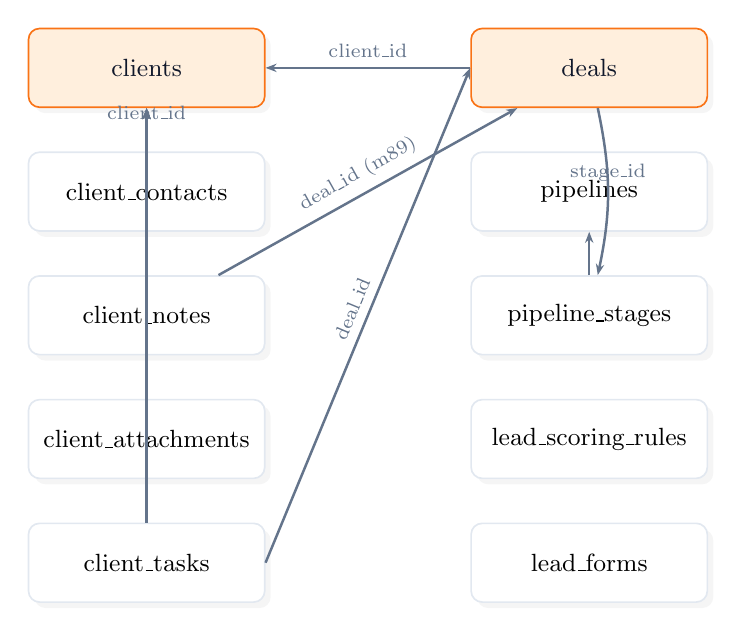
\begin{tikzpicture}[node distance=0.55cm and 1.2cm]
  \node[tcAccentBox, minimum width=3cm] (client) {clients};
  \node[tcBox, below=of client, minimum width=3cm] (contacts) {client\_contacts};
  \node[tcBox, below=of contacts, minimum width=3cm] (notes) {client\_notes};
  \node[tcBox, below=of notes, minimum width=3cm] (attach) {client\_attachments};
  \node[tcBox, below=of attach, minimum width=3cm] (ctasks) {client\_tasks};

  \node[tcAccentBox, right=2.6cm of client, minimum width=3cm] (deal) {deals};
  \node[tcBox, below=of deal, minimum width=3cm] (pipe) {pipelines};
  \node[tcBox, below=of pipe, minimum width=3cm] (stage) {pipeline\_stages};
  \node[tcBox, below=of stage, minimum width=3cm] (lsr) {lead\_scoring\_rules};
  \node[tcBox, below=of lsr, minimum width=3cm] (form) {lead\_forms};

  \draw[tcArrow] (contacts) -- node[font=\scriptsize\color{tcMuted},above]{client\_id} (client);
  \draw[tcArrow] (notes) -- (client);
  \draw[tcArrow] (attach) -- (client);
  \draw[tcArrow] (ctasks) -- (client);

  \draw[tcArrow] (deal) -- node[font=\scriptsize\color{tcMuted},above]{client\_id} (client);
  \draw[tcArrow] (notes) -- node[font=\scriptsize\color{tcMuted},above,sloped]{deal\_id (m89)} (deal);
  \draw[tcArrow] (ctasks.east) -- node[font=\scriptsize\color{tcMuted},sloped,above]{deal\_id} (deal.west);
  \draw[tcArrow] (stage) -- (pipe);
  \draw[tcArrow] (deal) edge[bend left=12] node[font=\scriptsize\color{tcMuted},above]{stage\_id} (stage);

\end{tikzpicture}
\caption{Client / deal relational map. Solid arrows are foreign keys.
The dashed lines around \texttt{notes \(\to\) deals} and
\texttt{client\_tasks \(\to\) deals} indicate optional links: a note or
task may belong only to a client without a specific deal.}
\label{fig:crm-erd}
\end{figure}

\subsection{Category field and grouping}

Client \textbf{Category} was added in migration~086. It is a nullable
text column with no enumeration; the form provides a free-text input
with an HTML5 \texttt{datalist} of common suggestions (Enterprise,
SMB, Startup, NGO, Government, Reseller, Agency, Education). The
Clients page surfaces the category in three places:

\begin{enumerate}[leftmargin=*,itemsep=2pt]
  \item As a secondary badge on every client card (dashed
    \emph{+ Category} placeholder when null, so the affordance is
    discoverable).
  \item As a dropdown filter in the toolbar (always rendered; when no
    categories exist, the menu shows a helper line).
  \item As a \emph{Group by category} toggle that switches the flat
    grid into one section per category, alphabetical, with
    \emph{Uncategorized} pinned to the bottom.
\end{enumerate}

After a successful CSV import, if any imported row has a category set
the page auto-flips to the grouped view and resets the category filter
to \emph{All} so every section is visible — surfaced via a toast.

\subsection{CSV import — extensibility}

The importer accepts the canonical 41-column template
(\texttt{CLIENT\_CSV\_HEADERS} in
\texttt{src/services/supabase/clients.ts}) and additionally lets the
user opt-in to capture extra columns into the client's
\texttt{custom\_fields} JSONB. The flow:

\begin{enumerate}[leftmargin=*,itemsep=2pt]
  \item User drops a CSV. We parse with Papaparse and run
    \texttt{previewClientImportRows}, which returns
    \texttt{\{importableRows, invalidRows, duplicateRows,
    unknownHeaders\}}.
  \item In the preview step the user can:
    \begin{itemize}[itemsep=0pt]
      \item Manually add custom column names that aren't in the
        canonical template.
      \item Quick-add chips for any \texttt{unknownHeaders} detected.
      \item Override duplicates row-by-row to create as new clients.
    \end{itemize}
  \item On commit, \texttt{importClientsFromCsv(org, user, name, rows,
    extraCustomColumns)} writes each row using
    \texttt{crm\_create\_client\_rpc} which respects org membership
    and the viewer-readonly policy from migration~043.
\end{enumerate}

\subsection{HubSpot-style record view}

The client detail drawer is a wide modal (95\% viewport, capped at
1400px) with a three-column layout that mirrors HubSpot's record page:

\begin{figure}[H]
\centering
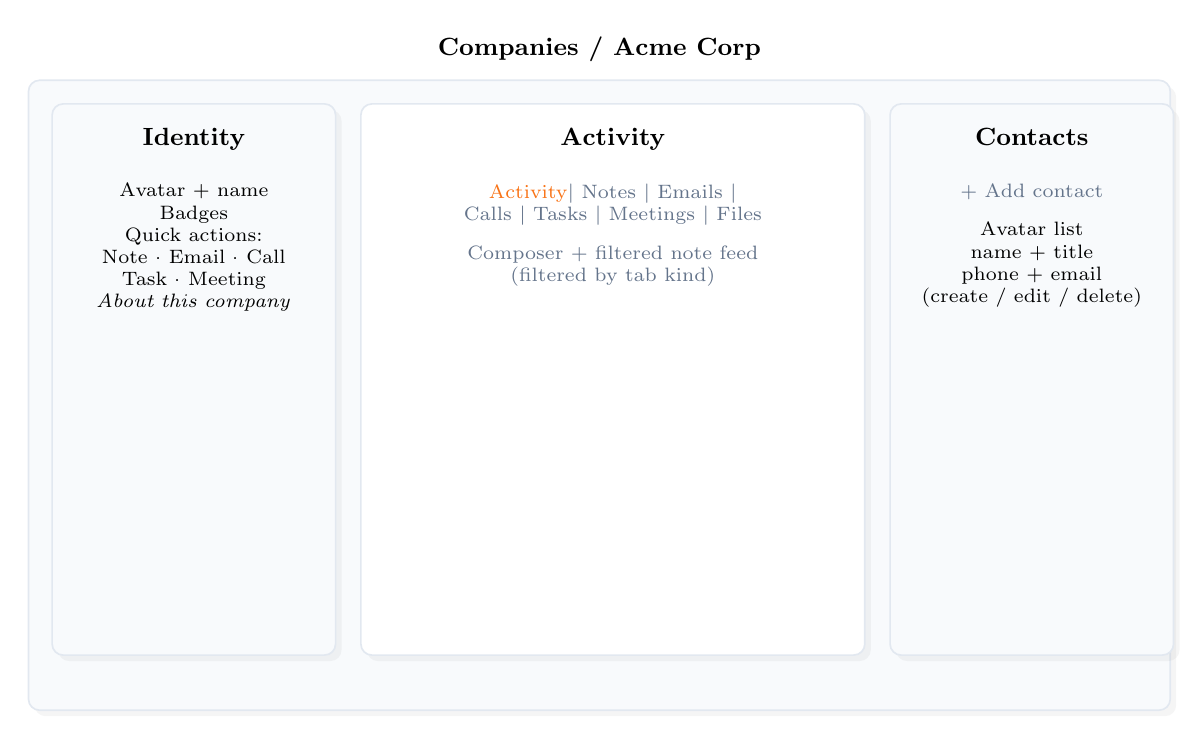
\begin{tikzpicture}[node distance=0.4cm and 0.5cm]

  % Outer modal
  \node[tcMutedBox, minimum width=14.5cm, minimum height=8cm] (modal) {};
  \node[above=0.1cm of modal.north, font=\small] {\textbf{Companies / Acme Corp}};

  % Left column
  \node[tcBox, anchor=north west, fill=tcBg, minimum width=3.6cm, minimum height=7cm]
    (left) at ([xshift=0.3cm, yshift=-0.3cm] modal.north west) {};
  \node[anchor=north, font=\small\bfseries] at ([yshift=-0.2cm] left.north) {Identity};
  \node[anchor=north, font=\scriptsize, align=center, text width=3.2cm]
    at ([yshift=-0.9cm] left.north)
    {Avatar + name\\Badges\\Quick actions:\\Note · Email · Call\\Task · Meeting\\\textit{About this company}};

  % Middle column
  \node[tcBox, anchor=north west, fill=white, minimum width=6.4cm, minimum height=7cm]
    (mid) at ([xshift=0.3cm] left.north east) {};
  \node[anchor=north, font=\small\bfseries] at ([yshift=-0.2cm] mid.north) {Activity};
  \node[anchor=north, font=\scriptsize, align=center, text width=6cm]
    at ([yshift=-0.9cm] mid.north)
    {\color{tcAccent}Activity\color{tcMuted} \textbar{} Notes \textbar{} Emails \textbar{} Calls \textbar{} Tasks \textbar{} Meetings \textbar{} Files\\[6pt]
    Composer + filtered note feed\\(filtered by tab kind)};

  % Right column
  \node[tcBox, anchor=north west, fill=tcBg, minimum width=3.6cm, minimum height=7cm]
    (right) at ([xshift=0.3cm] mid.north east) {};
  \node[anchor=north, font=\small\bfseries] at ([yshift=-0.2cm] right.north) {Contacts};
  \node[anchor=north, font=\scriptsize, align=center, text width=3.2cm]
    at ([yshift=-0.9cm] right.north)
    {{\color{tcMuted}+ Add contact}\\[6pt]Avatar list\\name + title\\phone + email\\(create / edit / delete)};

\end{tikzpicture}
\caption{Client (and deal) record view layout. Same three-column shell
used for both \texttt{ClientDetailDrawer} and
\texttt{DealDetailDrawer}; the right column shows contacts for clients
and the linked client card for deals.}
\label{fig:hubspot-layout}
\end{figure}

\subsection{Deal record view and per-deal notes}

The deal drawer uses the same three-column shell. Quick actions
(Note, Email, Call, Task, Meeting) open the matching sub-tab; Email and
Call additionally carry \texttt{mailto:} and \texttt{tel:} hrefs to the
linked client's contact so the user's default app launches with the
right address. Activity logged in the middle column is scoped to that
specific deal via the new \texttt{client\_notes.deal\_id} column
(migration~089). Each created note also carries \texttt{client\_id}
from the deal's linked client, so it appears on both the deal's feed
and the client's full timeline.

% ──────────────────────────────────────────────────────────────────────────
\section{The Automation engine}\label{sec:automation}

The automation engine is TaskCalendar's productivity multiplier and the
foundation that the AI Sales Agent (Section~\ref{sec:ai-agent}) and
Sequences run on top of. It mirrors Monday.com's recipe builder
(\emph{when X happens, do Y}) but adds tighter loop-prevention and a
pluggable action registry.

\subsection{Data model}

Four tables (migration 065):

\begin{itemize}[leftmargin=*,itemsep=2pt]
  \item \texttt{automation\_recipes} — the user-defined rules. Carries
    name, description, \texttt{trigger\_type}, \texttt{trigger\_config},
    \texttt{conditions[]}, \texttt{actions[]}, enabled flag,
    \texttt{run\_count}, \texttt{fail\_count}, \texttt{last\_run\_at}.
  \item \texttt{automation\_events} — the event queue.
    \texttt{event\_type}, \texttt{payload}, \texttt{source\_table},
    \texttt{source\_id}, \texttt{depth}, \texttt{enqueued\_at},
    \texttt{processed\_at}.
  \item \texttt{automation\_runs} — per-recipe execution log.
    \texttt{status} (success / failure / skipped / partial),
    \texttt{action\_results} (JSONB array), \texttt{started\_at},
    \texttt{finished\_at}.
  \item \texttt{automation\_worker\_heartbeat} — singleton row holding
    \texttt{last\_run\_at}, \texttt{last\_batch\_size},
    \texttt{last\_duration\_ms} for health monitoring.
\end{itemize}

\subsection{Trigger \(\to\) Action flow}

\begin{figure}[H]
\centering
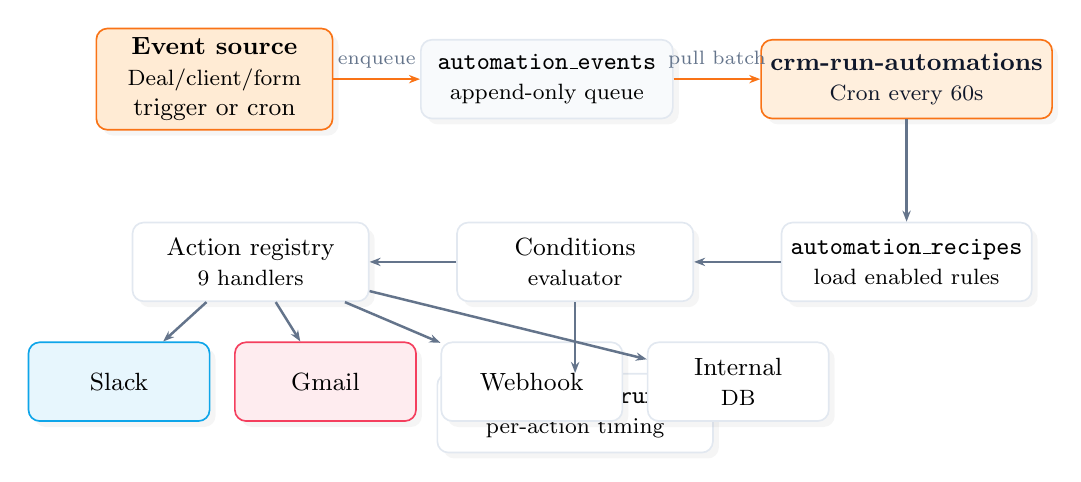
\begin{tikzpicture}[node distance=0.9cm and 1.1cm]

  % Triggers (input)
  \node[tcBox, fill=tcAccentSoft!50, draw=tcAccent, minimum width=3cm] (trigger) {\textbf{Event source}\\\footnotesize Deal/client/form\\trigger or cron};

  % Event queue
  \node[tcMutedBox, right=of trigger, minimum width=3.2cm] (queue) {\texttt{automation\_events}\\\footnotesize append-only queue};

  % Worker
  \node[tcAccentBox, right=of queue, minimum width=3cm] (worker) {\textbf{crm-run-automations}\\\footnotesize Cron every 60s};

  % Recipes
  \node[tcBox, below=1.3cm of worker, minimum width=3cm] (recipes) {\texttt{automation\_recipes}\\\footnotesize load enabled rules};

  % Conditions evaluator
  \node[tcBox, left=of recipes, minimum width=3cm] (cond) {Conditions\\\footnotesize evaluator};

  % Action registry
  \node[tcBox, left=of cond, minimum width=3cm] (actions) {Action registry\\\footnotesize 9 handlers};

  % Run log
  \node[tcBox, below=of cond, minimum width=3.5cm] (runs) {\texttt{automation\_runs}\\\footnotesize per-action timing};

  % External targets
  \node[tcBox, draw=tcSky, fill=tcSky!10, below left=0.5cm and -1cm of actions]
    (slack) {Slack};
  \node[tcBox, draw=tcRose, fill=tcRose!10, right=0.3cm of slack] (gmail) {Gmail};
  \node[tcBox, fill=white, right=0.3cm of gmail] (webhook) {Webhook};
  \node[tcBox, fill=white, right=0.3cm of webhook] (db) {Internal\\\footnotesize DB};

  % Arrows
  \draw[tcAccentArrow] (trigger) -- node[font=\scriptsize\color{tcMuted},above]{enqueue} (queue);
  \draw[tcAccentArrow] (queue) -- node[font=\scriptsize\color{tcMuted},above]{pull batch} (worker);
  \draw[tcArrow] (worker) -- (recipes);
  \draw[tcArrow] (recipes) -- (cond);
  \draw[tcArrow] (cond) -- (actions);
  \draw[tcArrow] (cond) -- (runs);

  \draw[tcArrow] (actions) -- (slack);
  \draw[tcArrow] (actions) -- (gmail);
  \draw[tcArrow] (actions) -- (webhook);
  \draw[tcArrow] (actions) -- (db);

\end{tikzpicture}
\caption{Automation engine flow. A trigger (DB AFTER UPDATE/INSERT
trigger, form submission, or cron tick) enqueues an event. The worker
pulls in batches of \(\le 200\), loads recipes whose
\texttt{trigger\_type} matches, evaluates conditions, and dispatches
each action through the registry. Outcomes are written to
\texttt{automation\_runs}.}
\label{fig:automation-flow}
\end{figure}

\subsection{Trigger catalogue}

\begin{table}[H]
\centering
\begin{tabular}{@{}p{3.7cm}p{3.5cm}p{6.5cm}@{}}
\toprule
\textbf{Trigger} & \textbf{event\_type} & \textbf{Source} \\
\midrule
Deal entered stage      & \texttt{deal\_stage\_entered}      & \texttt{deals} AFTER UPDATE trigger \\
Deal score band changed & \texttt{deal\_score\_band\_changed}& \texttt{clients} AFTER UPDATE \\
Deal field changed      & \texttt{deal\_field\_changed}      & \texttt{deals} AFTER UPDATE (whitelisted columns only) \\
Form submitted          & \texttt{form\_submitted}           & \texttt{form\_submissions} AFTER INSERT \\
Client created          & \texttt{client\_created}           & \texttt{clients} AFTER INSERT \\
Client tagged           & \texttt{client\_tagged}            & \texttt{clients} AFTER UPDATE (per added tag) \\
Task overdue            & \texttt{task\_overdue}             & cron sweep — newly overdue rows \\
Scheduled time          & \texttt{scheduled}                 & cron — cron expression on recipe config \\
\bottomrule
\end{tabular}
\caption{Eight triggers map to event types the worker subscribes to.
Database triggers are written in plpgsql with a watched-column
whitelist on UPDATE to suppress no-op fires.}
\end{table}

\subsection{Action catalogue}

\begin{table}[H]
\centering
\begin{tabular}{@{}p{3.3cm}p{4.5cm}p{6cm}@{}}
\toprule
\textbf{Action} & \textbf{Handler file} & \textbf{Behaviour} \\
\midrule
Create task       & \texttt{actions/createTask.ts}     & Resolves assignee placeholder
   (\texttt{deal\_owner} / \texttt{client\_owner} / uuid) \(\to\) user id; inserts into
   \texttt{client\_tasks} or \texttt{tasks}; optional dedupe key. \\
Tag client        & \texttt{actions/tagClient.ts}      & Add or remove a tag from
   \texttt{clients.tags}. \\
Set field         & \texttt{actions/setField.ts}       & Whitelisted column update
   on \texttt{deal} or \texttt{client}. \\
Change owner      & \texttt{actions/changeOwner.ts}    & Updates owner id AND
   denormalised owner name. \\
Add note          & \texttt{actions/addNote.ts}        & Inserts a \texttt{client\_notes}
   row authored as ``Automation: \emph{recipe name}''. Supports
   \verb|{{placeholders}}|. \\
Move deal stage   & \texttt{actions/moveDealStage.ts}  & Resolves
   \texttt{next} / \texttt{previous} via \texttt{pipeline\_stages.position};
   surfaces gating-trigger errors verbatim. \\
Webhook POST      & \texttt{actions/webhook.ts}        & HMAC-SHA256 signed POST
   with SSRF allowlist; 30\,s timeout. \\
Slack message     & \texttt{actions/slackPost.ts}      & Routes through
   \texttt{integrations-action} edge function. Skipped if no active
   Slack integration. \\
Send email        & \texttt{actions/sendEmail.ts}      & Routes through
   \texttt{integrations-action}; uses connected user's Gmail. \\
\bottomrule
\end{tabular}
\caption{Action registry. Each handler returns
\texttt{\{status, message?, meta?\}}; the per-recipe runner stops on
first failure and downgrades to \texttt{partial} on \texttt{skipped}.}
\end{table}

\subsection{Template substitution}

Any action that accepts text (Add note subject, Webhook URL, Slack
message body, Send email body) supports mustache-style placeholders
resolved by \texttt{shared/substitute.ts}:

\begin{lstlisting}[language=TypeScript]
substitute("Deal {{deal.title}} won — value {{deal.value}} {{deal.currency}}", ctx)
//   ↳  "Deal Acme Pilot won — value 24000 GBP"
\end{lstlisting}

Resolvable variables include \verb|{{deal.title}}|,
\verb|{{deal.value}}|, \verb|{{deal.currency}}|, \verb|{{deal.stage}}|,
\verb|{{deal.url}}|, \verb|{{client.name}}|, \verb|{{client.email}}|,
\verb|{{client.industry}}|, \verb|{{client.url}}|, \verb|{{actor}}|,
\verb|{{recipe.name}}|. Unknown placeholders pass through unchanged.

\subsection{Loop prevention and safety}

The engine's primary loop guard is \textbf{per-recipe burst detection}:
before evaluating any recipe, the worker counts that recipe's
\texttt{automation\_runs} in the past 60 seconds. If the count is
\(\ge\) 100, the worker auto-disables the recipe
(\texttt{enabled=false}) and writes a \texttt{skipped} run with
message \texttt{auto\_disabled\_runaway}. A secondary 1000-runs / 24h
ceiling catches slower loops.

\begin{table}[H]
\centering
\begin{tabular}{@{}lll@{}}
\toprule
\textbf{Defence} & \textbf{Window} & \textbf{Outcome} \\
\midrule
Burst detection      & 60 s   & Auto-disable + admin notification \\
Daily ceiling        & 24 h   & \texttt{skipped}: rate\_limited \\
Webhook rate limit   & 1 min  & In-memory bucket, 60 calls / org \\
\texttt{depth} breadcrumb & per-event & Worker writes \texttt{event.depth+1} on spawned events (advisory only) \\
\bottomrule
\end{tabular}
\caption{Loop and abuse defences.}
\end{table}

\subsection{Worker concurrency}

A PostgreSQL advisory lock (\texttt{pg\_try\_advisory\_lock(0xC8AE0001)})
serialises worker invocations. The cron schedule fires every minute; if
a previous run is still in flight, the new invocation exits
immediately with \texttt{skipped: already\_running}. A typical run
processes \(\le 200\) events at \(\sim 50\,\text{ms}\) each, comfortably
within the 5-minute Edge Function ceiling.

\subsection{Recipe UI}

The Recipe Builder modal lives at \emph{Settings \(\to\) Automations}
(admin-gated and \texttt{crm}-feature-gated). A recipe draft has the
shape:

\begin{lstlisting}[language=TypeScript]
interface RecipeDraft {
  name: string;
  enabled: boolean;
  trigger: { type: TriggerType; config: Record<string, unknown> };
  conditions: Array<{ field: string; operator: string; value: unknown }>;
  actions: Array<{ type: ActionType; config: Record<string, unknown> }>;
}
\end{lstlisting}

A live-run toast (Sonner) fires on every
\texttt{automation\_runs} INSERT via Realtime, so admins see recipes
firing in real time across their organisation.

% ──────────────────────────────────────────────────────────────────────────
\section{AI building blocks}

\subsection{AI Blocks}

AI Blocks are reusable LLM-backed action handlers that plug into the
automation engine. Three handlers are spec'd: \texttt{aiSummarize},
\texttt{aiClassify}, \texttt{aiDraftEmail}. Each accepts a small
\texttt{config} and a substituted prompt, calls the OpenAI completions
API server-side via the \texttt{ai-chat} edge function, and writes the
result either back into \texttt{client\_notes} (for review) or
directly into a deal/client field via \texttt{setField}.

\subsection{AI Sales Agent}\label{sec:ai-agent}

The AI Sales Agent is a daemon process that scans the org's pipeline
for opportunities and posts suggestions. Examples:

\begin{itemize}[leftmargin=*,itemsep=2pt]
  \item \emph{Acme Corp opened your proposal 4× today. Want me to
    draft a follow-up?}
  \item \emph{Deal Globex hasn't moved in 12 days — snooze or reach
    out?}
  \item \emph{Lead score climbed for Initech (62 \(\to\) 84)}.
\end{itemize}

Every suggestion is gated behind a \emph{Review} / \emph{Approve}
button — nothing sends without an admin tap. Approval triggers a
matching automation action (e.g., \texttt{addNote} + \texttt{sendEmail}).

% ──────────────────────────────────────────────────────────────────────────
\section{Chat-bot integrations}

The two chat-bot adapters share a common platform-agnostic core under
\texttt{supabase/functions/\_shared/agent/}:

\begin{itemize}[leftmargin=*,itemsep=2pt]
  \item \texttt{types.ts} — \texttt{Intent}, \texttt{AgentReply},
    \texttt{PendingAction}, \texttt{LinkedAccount}.
  \item \texttt{intent.ts} — OpenAI-backed parser; receives the
    user's text plus the org's workspace / project / client names and
    returns a structured \texttt{Intent}.
  \item \texttt{agentActions.ts} — provider-parameterised resolver +
    executor. Reads the parsed \texttt{Intent}, resolves entity names
    \(\to\) ids, queues an \texttt{agent\_pending\_actions} row for the
    confirm step, and dispatches to one of five
    \texttt{agent\_create\_*} SECURITY DEFINER RPCs on confirm.
\end{itemize}

\subsection{Conversation flow}

\begin{figure}[H]
\centering
\begin{tikzpicture}[node distance=0.7cm and 0.95cm]

  \node[tcBox, fill=tcAccentSoft!40, draw=tcAccent, minimum width=2.6cm] (user) {User};
  \node[tcBox, draw=tcSky, fill=tcSky!10, right=of user, minimum width=2.4cm] (tg) {Telegram /\\WhatsApp};
  \node[tcBox, right=of tg, minimum width=2.8cm] (hook) {Webhook\\Edge Function};
  \node[tcBox, right=of hook, minimum width=2.6cm, draw=tcViolet, fill=tcViolet!10] (llm) {OpenAI\\intent parse};
  \node[tcBox, below=1.2cm of hook, minimum width=2.8cm] (pending) {agent\_pending\_actions};
  \node[tcBox, left=of pending, minimum width=2.8cm] (convo) {agent\_conversation\_state};
  \node[tcBox, right=of pending, minimum width=2.8cm] (rpc) {agent\_create\_* RPC};
  \node[tcAccentBox, right=of rpc, minimum width=2.4cm] (db) {Postgres\\insert};

  \draw[tcAccentArrow] (user) -- node[font=\scriptsize\color{tcMuted},above]{/start <code>} (tg);
  \draw[tcArrow] (tg) -- node[font=\scriptsize\color{tcMuted},above]{HTTPS POST} (hook);
  \draw[tcArrow] (hook) -- node[font=\scriptsize\color{tcMuted},above]{text + ctx} (llm);
  \draw[tcArrow] (llm) -- node[font=\scriptsize\color{tcMuted},below,sloped]{Intent} (hook);
  \draw[tcArrow] (hook) -- (pending);
  \draw[tcArrow] (hook) -- node[font=\scriptsize\color{tcMuted},sloped,above]{missing field} (convo);
  \draw[tcArrow] (hook) edge[bend left=20] node[font=\scriptsize\color{tcMuted},above]{Confirm card} (tg);
  \draw[tcArrow] (tg) edge[bend right=20] node[font=\scriptsize\color{tcMuted},below]{tap ✅} (hook);
  \draw[tcArrow] (pending) -- (rpc);
  \draw[tcArrow] (rpc) -- (db);
  \draw[tcArrow] (hook) edge[bend right=12] node[font=\scriptsize\color{tcMuted},below,sloped]{✓ Created} (tg);
  \draw[tcArrow] (tg) edge[bend right=15] (user);

\end{tikzpicture}
\caption{Chat-bot conversation flow. The user always speaks first.
Every create is buffered in \texttt{agent\_pending\_actions} and only
materialises when the user taps the confirm button. Missing fields
are tracked in \texttt{agent\_conversation\_state} so a single-word
follow-up like ``Marketing'' fills the prompt without re-parsing.}
\label{fig:bot-flow}
\end{figure}

\subsection{Telegram adapter}

Telegram is the simpler of the two:
\begin{itemize}[leftmargin=*,itemsep=2pt]
  \item Auth: secret-token header (\texttt{X-Telegram-Bot-Api-Secret-Token})
    plus a path-segment secret on the webhook URL.
  \item Linking: 6-digit code from \emph{Settings \(\to\)
    Integrations \(\to\) Telegram}; the bot consumes the code on
    \texttt{/start <code>}.
  \item Identity: Telegram \texttt{user.id} stored as the
    \texttt{external\_id} on the \texttt{integrations.metadata}.
\end{itemize}

\subsection{WhatsApp adapter}

WhatsApp follows the same shape but with Meta's specifics:
\begin{itemize}[leftmargin=*,itemsep=2pt]
  \item Auth: HMAC-SHA256 signature on the request body, signed with
    the Meta App Secret, sent in \texttt{X-Hub-Signature-256}.
    Constant-time compare.
  \item Linking: 6-digit code, same flow. Bot replies via
    interactive reply buttons (max 3) — perfect for Confirm /
    Cancel / Edit.
  \item Identity: E.164 phone number stored as \texttt{external\_id}
    plus \texttt{current\_org\_id} in metadata.
  \item Subscription: two-step. App-level \texttt{messages} field
    subscription via Meta UI, \emph{and} WABA \(\to\) App subscription
    via \texttt{POST /v20.0/<waba\_id>/subscribed\_apps}. The latter
    is the gotcha that bit us during deployment.
\end{itemize}

\subsection{Confirm-before-write pattern}

For both platforms, every entity-creation action follows the same
pattern:

\begin{enumerate}[leftmargin=*,itemsep=2pt]
  \item User sends a message.
  \item Webhook resolves the user, fetches a compact org-scoped
    context (workspace / project / client names), forwards to OpenAI.
  \item OpenAI returns a structured \texttt{Intent}.
  \item Resolver looks up entity ids; on ambiguity returns a
    \emph{choices} reply.
  \item On clean resolution, queues a row in
    \texttt{agent\_pending\_actions} (10-minute TTL) and replies
    with a Confirm / Cancel inline-button card.
  \item User taps Confirm \(\to\) webhook calls the matching
    \texttt{agent\_create\_*} RPC; deletes the pending row; replies
    with success.
\end{enumerate}

% ──────────────────────────────────────────────────────────────────────────
\section{Google integrations}

\subsection{Google Meet attached to tasks}

When creating or editing a task, a checkbox \emph{Add Google Meet
link} appears under the date picker (requires Google connected
\emph{and} a due date set). The meeting time is picked separately via
an \texttt{<input type="time">}; the start datetime is composed from
the date + time and sent to a dedicated edge function
\texttt{task-create-meet} which:

\begin{enumerate}[leftmargin=*,itemsep=2pt]
  \item Verifies the caller is a member of the task's organisation
    via \texttt{is\_org\_member\_for}.
  \item Decrypts the user's Google OAuth access token (AES-256-GCM
    at rest, refreshes if expiring \(<60\,\text{s}\)).
  \item Calls \texttt{POST /calendar/v3/calendars/primary/events?conferenceDataVersion=1}
    with a \texttt{hangoutsMeet} conference request.
  \item Writes the returned \texttt{hangoutLink} and \texttt{eventId}
    back to the \texttt{tasks} row.
  \item If the caller passed an explicit \texttt{startTime}, the task's
    \texttt{due\_date} is updated to match so the UI stays consistent.
\end{enumerate}

\subsection{Gmail send}

Gmail is invoked from the automation engine's \texttt{sendEmail}
action and (planned) from the task-assignment notification path.
Scope: \texttt{gmail.send} only — never \texttt{readonly} or
\texttt{modify}.

% ──────────────────────────────────────────────────────────────────────────
\section{Subscription plans and gating}\label{sec:plans}

\subsection{Tiers}

\begin{table}[H]
\centering
\small
\begin{tabular}{@{}lp{2.4cm}lp{6.4cm}@{}}
\toprule
\textbf{Plan} & \textbf{Audience} & \textbf{Price (GBP)} & \textbf{Highlights} \\
\midrule
Starter  & Solo trial     & Free              & 3 projects, 20 tasks/project, 1 workspace, 1 member. \\
Basic    & Students / individuals & 5–7.99 / mo & 15 projects, unlimited tasks, 3 workspaces, 3 members, 5 GB, AI assistant, time tracking. \\
Advanced & Teams up to 10 & 45–50 / mo + 2.99 / extra member & Everything in Basic + Team collab, Advanced analytics, Timeline, Contracts, \textbf{CRM}, \textbf{Automation}, \textbf{AI Sales Agent}. \\
Premium  & Enterprises    & Custom            & Unlimited everything + API access + custom integrations. \\
\bottomrule
\end{tabular}
\end{table}

Trial: every new sign-up gets a 28-day full-Advanced trial (no card).
Day 29: auto-downgrade to Starter unless they've subscribed.

\subsection{Feature gating diagram}

\begin{figure}[H]
\centering
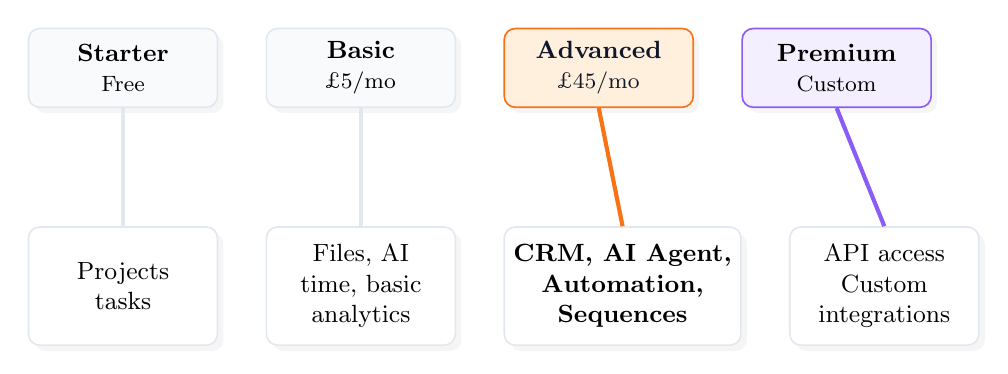
\begin{tikzpicture}[node distance=0.5cm and 0.6cm]

  % Plans
  \node[tcMutedBox, minimum width=2.4cm] (starter) {\textbf{Starter}\\\footnotesize Free};
  \node[tcMutedBox, right=of starter, minimum width=2.4cm] (basic) {\textbf{Basic}\\\footnotesize £5/mo};
  \node[tcAccentBox, right=of basic, minimum width=2.4cm] (adv) {\textbf{Advanced}\\\footnotesize £45/mo};
  \node[tcBox, right=of adv, draw=tcViolet, fill=tcViolet!10, minimum width=2.4cm] (prem) {\textbf{Premium}\\\footnotesize Custom};

  % Feature blocks
  \node[tcBox, below=1.5cm of starter, minimum width=2.4cm, minimum height=1.5cm]
    (proj) {Projects\\tasks};
  \node[tcBox, right=of proj, minimum width=2.4cm, minimum height=1.5cm]
    (pm) {Files, AI\\time, basic\\analytics};
  \node[tcBox, right=of pm, minimum width=2.4cm, minimum height=1.5cm]
    (crm) {\textbf{CRM, AI Agent,}\\\textbf{Automation,}\\\textbf{Sequences}};
  \node[tcBox, right=of crm, minimum width=2.4cm, minimum height=1.5cm]
    (api) {API access\\Custom\\integrations};

  % Inclusion brackets
  \draw[tcLight, line width=1.5pt] (starter.south) -- (proj.north);
  \draw[tcLight, line width=1.5pt] (basic.south) -- (pm.north);
  \draw[tcAccent, line width=1.5pt] (adv.south) -- (crm.north);
  \draw[tcViolet, line width=1.5pt] (prem.south) -- (api.north);

\end{tikzpicture}
\caption{Feature ladder. Each tier inherits everything below it. The
\texttt{crm} feature umbrella gates the Clients page, AI Sales Agent,
Automations, Sequences, Pipelines, Lead scoring, Lead forms, and the
CRM analytics dashboard.}
\label{fig:plans}
\end{figure}

\subsection{Where gates are enforced}

\begin{enumerate}[leftmargin=*,itemsep=2pt]
  \item \textbf{ProtectedRoute}. Routes can declare
    \texttt{requireFeature="crm"}; locked users are redirected to
    \texttt{/pricing}. Wired on \texttt{/clients},
    \texttt{/clients/activity}, \texttt{/ai-agent},
    \texttt{/dashboard/clients}.
  \item \textbf{Sidebar}. Quick-menu items filter by
    \texttt{hasFeature(...)}; the CRM analytics entry hides on Basic.
  \item \textbf{Settings tabs}. The whole CRM and Automation tab
    sections only render when \texttt{hasFeature('crm')}.
  \item \textbf{Plan caps}. \texttt{usePlanLimits} checks project,
    task, and member counts before writes; the
    \texttt{LimitReachedModal} explains the upgrade path.
\end{enumerate}

% ──────────────────────────────────────────────────────────────────────────
\section{Dashboards}

Two graphical dashboards built with Recharts share a small set of
primitives in \texttt{src/components/dashboards/}:

\begin{itemize}[leftmargin=*,itemsep=2pt]
  \item \texttt{KpiTile} — number + label + sparkline + delta-percent
    badge.
  \item \texttt{ChartCard} — uniform card shell.
  \item \texttt{StatusDonut}, \texttt{BarHorizontal},
    \texttt{StackedBar}, \texttt{TrendArea}, \texttt{PipelineFunnel} —
    chart wrappers.
\end{itemize}

The palette is monochrome (slate-400 default, with grey shades for
categorical series) plus a single orange accent (\#F97316) reserved
for the focal series (current period, won stage, top performer).

\subsection{Projects analytics dashboard}

KPIs: active tasks, completed in the selected range, overdue, average
cycle time. Charts: task status donut, throughput stacked bar (created
vs completed, 14 days), workload by assignee horizontal bar (top 10),
project completion list (top 8 by \% done with overdue badge).

\subsection{CRM analytics dashboard}

KPIs: open deals (count + value), won this period with delta vs
previous period, win rate, average deal cycle. Charts: pipeline funnel
(counts + value per stage), weighted forecast (next 6 months), top
performers horizontal bar, lead-score donut (hot/warm/cold), deals at
risk list (stalled \(\ge 14\,\text{days}\)), activity by type
horizontal bar.

% ──────────────────────────────────────────────────────────────────────────
\section{Security and data handling}

\subsection{Authentication}

Firebase Auth provides identity; tokens are exchanged for a Supabase
JWT signed with the project's anon key. Every PostgreSQL session
inherits the JWT's claims, including \texttt{sub} (mapped to
\texttt{auth.uid()}) and \texttt{role} (\texttt{authenticated} for
end users, \texttt{service\_role} for Edge Functions using the
service-role key).

\subsection{Row-Level Security}

Every domain table enables RLS. The recurring pattern:

\begin{lstlisting}[language=TypeScript, frame=lines]
create policy "org members read X"
  on public.X for select
  using (public.is_org_member(organization_id));
\end{lstlisting}

Writes either:
\begin{itemize}[leftmargin=*,itemsep=2pt]
  \item Go through a \texttt{SECURITY DEFINER} RPC that re-checks
    membership using \texttt{auth.uid()}; or
  \item Are performed by the service role from an Edge Function,
    where membership is re-checked via
    \texttt{is\_org\_member\_for(p\_user\_id, p\_org\_id)}.
\end{itemize}

\subsection{OAuth token storage}

Provider access tokens are encrypted at rest with AES-256-GCM
(\texttt{INTEGRATION\_TOKEN\_KEY}). The browser never receives the
plaintext; Edge Functions decrypt on demand for outbound calls and
refresh tokens that are within 60\,s of expiry.

\subsection{Bot-specific guards}

\begin{itemize}[leftmargin=*,itemsep=2pt]
  \item Webhook signature verification (Telegram secret token;
    WhatsApp HMAC) — constant-time compare on both.
  \item Link codes are 6-digit, SHA-256 hashed at rest, single-use,
    10-minute TTL, 5-per-hour rate limit per user.
  \item Service-role calls re-evaluate org membership via
    \texttt{is\_org\_member\_for} before any write.
  \item Webhook returns \texttt{200} on internal exceptions to stop
    Meta / Telegram retry amplification; errors are surfaced via the
    chat reply or the Edge Function log.
\end{itemize}

\subsection{Workforce clock}

The \texttt{ClockGate} component forces every signed-in
\textbf{Admin} or \textbf{Member} to clock in before the app renders.
Org Owners, Viewers, and the app-owner bypass. A 9-hour cutoff
auto-closes any open entry via the cron-scheduled
\texttt{close\_stale\_time\_entries(9)} function — relevant when a
user forgets to clock out at end of day.

% ──────────────────────────────────────────────────────────────────────────
\section{Database schema summary}

\begin{table}[H]
\centering
\footnotesize
\begin{tabular}{@{}lp{5cm}lp{4cm}@{}}
\toprule
\textbf{Domain} & \textbf{Tables} & \textbf{Mig.} & \textbf{Notes} \\
\midrule
Core PM      & projects, tasks, workspaces, organizations, organization\_members & 001-022 & Multi-tenant base. \\
Integrations & integrations, integration\_events                            & 057     & Encrypted tokens. \\
CRM          & clients, client\_contacts, client\_notes, client\_attachments, client\_tasks & 041-044 & + \emph{category} 086, + \emph{deal\_id on notes} 089. \\
Deals        & deals, pipelines, pipeline\_stages                            & 045, 058 & Pipeline gating. \\
Lead scoring & lead\_scoring\_rules, lead\_scoring\_thresholds              & 060     & Auto-bucket cold/warm/hot. \\
Lead forms   & lead\_forms                                                   & 062     & Turnstile + dedup. \\
Automation   & automation\_recipes, automation\_events, automation\_runs, automation\_worker\_heartbeat & 065 & Cron-driven. \\
AI Blocks    & (action registry only — no new tables)                       & 066 & Pluggable handlers. \\
Sequences    & sequences, sequence\_runs                                     & 067     & Drip flows. \\
AI Agent     & ai\_agent\_settings, ai\_agent\_suggestions                  & 068     & Review-gated. \\
Telegram     & telegram\_link\_codes, agent\_pending\_actions, agent\_create\_* RPCs, agent\_conversation\_state & 082-085 & Chat-bot core. \\
WhatsApp     & whatsapp\_link\_codes (reuses agent\_pending\_actions)        & 088     & Same Intent core. \\
\bottomrule
\end{tabular}
\caption{Schema overview by domain, with the migrations that introduced
each set of tables.}
\end{table}

% ──────────────────────────────────────────────────────────────────────────
\section{Deployment and operations}

\subsection{Build and deploy}

\begin{itemize}[leftmargin=*,itemsep=2pt]
  \item Frontend: \texttt{npm run build} \(\to\) Vercel (preview +
    production environments). TypeScript strict mode; build fails on
    unused locals (TS6133), which has caught us at least three times
    on recent landing-page work.
  \item Edge Functions: \texttt{npx supabase functions deploy
    <name>}; the bot webhooks deploy with
    \texttt{--no-verify-jwt} because authentication is handled inside
    via secret-token (Telegram) or HMAC (WhatsApp).
  \item Migrations: \texttt{npx supabase db push} pushes any
    locally-pending file into \texttt{supabase\_migrations.schema\_migrations}.
    Filenames are version-keyed; a duplicate version produces a unique-
    constraint violation (rename to a fresh slot).
\end{itemize}

\subsection{Environment variables}

\begin{table}[H]
\centering
\small
\begin{tabular}{@{}p{4.6cm}p{3.6cm}p{6cm}@{}}
\toprule
\textbf{Variable} & \textbf{Surface} & \textbf{Purpose} \\
\midrule
\texttt{SUPABASE\_URL}                & both         & Edge functions and frontend. \\
\texttt{SUPABASE\_SERVICE\_ROLE\_KEY} & functions    & Server-side admin client. \\
\texttt{SUPABASE\_ANON\_KEY}          & both         & JWT verification. \\
\texttt{OPENAI\_API\_KEY}             & functions    & Intent parsing, AI agent, AI blocks. \\
\texttt{TELEGRAM\_BOT\_TOKEN}         & functions    & Telegram API auth. \\
\texttt{TELEGRAM\_WEBHOOK\_SECRET}    & functions    & Verifies inbound Telegram POSTs. \\
\texttt{WHATSAPP\_ACCESS\_TOKEN}      & functions    & Meta system-user permanent token. \\
\texttt{WHATSAPP\_PHONE\_NUMBER\_ID}  & functions    & Outbound sends. \\
\texttt{WHATSAPP\_VERIFY\_TOKEN}      & functions    & GET subscribe handshake. \\
\texttt{WHATSAPP\_APP\_SECRET}        & functions    & HMAC payload verification. \\
\texttt{INTEGRATION\_TOKEN\_KEY}      & functions    & AES-256-GCM key for stored tokens. \\
\texttt{SLACK\_SIGNING\_SECRET}       & functions    & Events API signature. \\
\texttt{VITE\_TELEGRAM\_BOT\_USERNAME}& frontend     & Settings card link. \\
\texttt{VITE\_WHATSAPP\_BOT\_NUMBER}  & frontend     & Settings card hint. \\
\bottomrule
\end{tabular}
\end{table}

% ──────────────────────────────────────────────────────────────────────────
\section{Conclusion}

TaskCalendar in its current form is a layered product. The base layer
is a competent project-management tool. The middle layer is a real CRM
with categorisable clients, multi-pipeline deals, lead capture, lead
scoring, and deal-scoped activity logging. The top layer is an
automation engine that ties everything together — fired by user
actions, cron, or chat-bot messages, and reaching out to Slack, Gmail,
Google Calendar/Meet, and arbitrary webhooks. Two chat-bot adapters
sit alongside, sharing a single \texttt{\_shared/agent} core so any
intent-parsing improvement upgrades both bots at once.

The architectural choices that matter most:
\begin{itemize}[leftmargin=*,itemsep=2pt]
  \item RLS-first writes with SECURITY DEFINER escape hatches only
    where strictly required.
  \item Confirm-before-write on the chat-bot path so an LLM can never
    write without an explicit user tap.
  \item One automation engine driving the AI Agent, Sequences, and
    AI Blocks rather than three parallel pipelines.
  \item A small set of dashboard primitives reused across the
    Projects and CRM dashboards, keeping look-and-feel consistent.
\end{itemize}

The roadmap from here is incremental rather than disruptive: more
trigger types in the automation engine, AI Blocks shipped from spec to
production, Sequences with wait/delay nodes, and template-message
support so the WhatsApp bot can initiate conversations outside the
24-hour window.

\vfill
\begin{center}
\small\color{tcMuted}
{\itshape Document generated 20 May 2026 \quad·\quad
Securovix Ltd, United Kingdom}
\end{center}

\end{document}
